\chapter{Aplikacja - symulator}
\label{ch:dodatekA-aplikacja}
\section{Założenia projektowe aplikacji}

\par
Aplikacja powstała w trakcie pracy miała umożliwić przeprowadzenie badań porównawczych algorytmu memetycznego z innymi algorytmami ewolucyjnymi. Zamiast udostępnienia możliwości ręcznego określenia konfiguracji algorytmów zdecydowano się na wykorzystanie opracowanych w pracy scenariuszy doboru atrybutów. 

\par
Przyjęte założenia projektowe aplikacji można podzielić na dwie kategorie:
\begin{itemize}
\item funkcjonalne:
\begin{itemize}
\item przeprowadzenie badań porównawczych w oparciu o cztery przyjęte kryteria,
\item selekcja parametrów algorytmu z wykorzystaniem zaproponowanych w pracy scenariuszy,
\item definiowanie własnych funkcji testowych:
\begin{itemize}
\item określanie parametrów funkcji, ich nazw i zakresu wartości,
\item generowanie szablonu kodu źródłowego,
\item zapisanie kodu źródłowego funkcji w języku \emph{R},
\end{itemize}
\item generowanie wykresów funkcji dwóch parametrów,
\end{itemize}
\item niefunkcjonalne:
\begin{itemize}
\item wykorzystanie implementacji algorytmów z popularnych pakietów języka \emph{R}
\item umożliwienie modyfikacji wykorzystanych w badaniach skryptów poprzez dostęp do nich.
\end{itemize}
\end{itemize}

\section{Instrukcja instalacyjna}

\par
Praca w całości została oparta o implementacje mechanizmów optymalizacji problemów rzeczywistoliczbowych dostępne w pakietach \emph{GA} i \emph{PSO} dla języka \emph{R}. Z tego powodu niezbędne do działania aplikacji jest instalacja interpretera języka \emph{R} oraz odpowiednia konfiguracja środowiska. Powstała aplikacja graficzna napisana została w języku \emph{Java} i jako interfejs \emph{Java}$Leftrightarrow$\emph{R} wykorzystuje bibliotekę \emph{JRI} po jednej stronie oraz pakiet \emph{rJava}.

\par
Proces przygotowania środowiska do działania można podzielić na następujące kroki:
\begin{enumerate}
\item pobranie i instalacja interpretera języka \emph{R},
\item uruchomienie interpretera i pobranie pakietu \emph{rJava} poleceniem \lstinline{install.packages("rJava")},
\item dodanie do zmiennej systemowej \lstinline{PATH} ścieżek do zaintalowanego interpretera oraz lokalizacji pakieru \emph{rJava}, dla systemów \emph{Windows} domyślnie:
\begin{itemize}
\item \lstinline{%HOMEPATH%\Documents\R\win-library\3.3\rJava\jri\x64}
\item \lstinline{C:\Program Files\R\R-3.3.3\bin\x64}
\end{itemize}
\item uruchomienie aplikacji i wywołanie najprostrzej operacji, np. generowanie wykresu \emph{Schaffer nr 2},
\item zatwierdzenie prośby o pobranie brakujących dodatkowych pakietów (wymaga połączenia z internetem)
\end{enumerate}
Po wykonaniu powyższej instrukcji można swobodnie korzystać z aplikacji. Jedynym obostrzeniem nałożonym na środowisko jest względne położenie pliku wykonywalnego aplikacji i dołączonego folderu zawierającego wykorzystywane skrypty w języku \emph{R}. 


\begin{table}[ht]
\caption{Poprawna wzajemna lokalizacja aplikacji i katalogu skryptów}
\label{table:app01-lokalizacja}
\begin{center}
\begin{tabular}{|l|}
	\hline
	{\lstinline[]$.\run.jar$} \\
	{\lstinline[]$.\javaEntryPoints\*.R$} \\
	\hline
	\end{tabular}
\end{center}
\end{table}





\section{Opis interfejsu graficznego}

\par
Wygląd aplikacji przedstawiono na rysunku \ref{fig:app01-fullScreen}. Interfejs można podzielić funkcjonalnie na 5 części oznaczonych \emph{A}, \emph{B}, \emph{C} i \emph{D} oraz osobno przedstawionej na rysunku \ref{fig:app01-plotTab}. 

\par
Sekcja \emph{A} pozwala na zdefiniowanie i wywołanie operacji. Możliwe jest uruchomienie zarówno procesu selekcji parametrów algorytmów jak i badań pod kątem jednego z kryteriów porównawczych użytych w pracy. Możliwy jest wybór spośród trzech funkcji testowych lub zdefiniowanej przez użytkownika - opcja \emph{(code)}. Lista z prawe strony panelu umożliwia na określenie, które z scenariuszy doboru parametrów powinny zostać użyte do selekcji. Możliwością dostępną jedynie w przypadku wykorzystania funkcji \emph{Schaffer nr 2} lub własnej funkcji z dwoma parametrami jest wygenerowanie jej wykresu w dziedzinie równej zakresowi poszczególnych atrybutów. 
 
\par
Panel oznaczony jako \emph{B} przedstawia bieżące konfiguracje algorytmów, które zostaną wykorzystane w przypadku uruchomienia badań porównawczych. Przy starcie aplikacji parametry wszystkich mechanizmów ustawiane są na te uzyskane w trakcie badań dla funkcji \emph{Schaffer nr 2}.

\par
Przedstawiona na rysunku \ref{fig:app01-fullScreen} sekcja \emph{C} przedstawia panel umożliwiający definiowanie własnych funkcji testowych. Górna część pozwala na określenie liczby, nazwy i zakresu parametrów. Przycisk \emph{Generate} tworzy pusty szablon w oparciu o określone parametry. Kod źródłowy opisujący nową funkcję należy zapisać w języku \emph{R}. W wskazanym polu edycji możliwe jest definiowanie dodatkowych pomocniczych funkcji jak również i dołączanie konkretnych pakietów. Nie można jednak modyfikować nazwy funkcji, ponieważ będzie to skutkowało niepoprawnym działaniem aplikacji. Zakładka \emph{code} aktywna jest jedynie wtedy, gdy w panelu \emph{A} wybrano opcję \emph{(code)}.

\par
Dolna część \emph{D} aplikacji stanowi narzędzie pomocnicze dla użytkownika. Zamieszczane są tam logi aplikacji umożliwiające rozwiązywanie problemów z poprawnością zdefiniowanej funkcji. Dodatkowo można znaleźć tam informacje dotyczące lokalizacji w systemie plików wykresów powstałych w skutek operacji z panelu \emph{A}. 


\begin{figure}[hbt]
\centering
  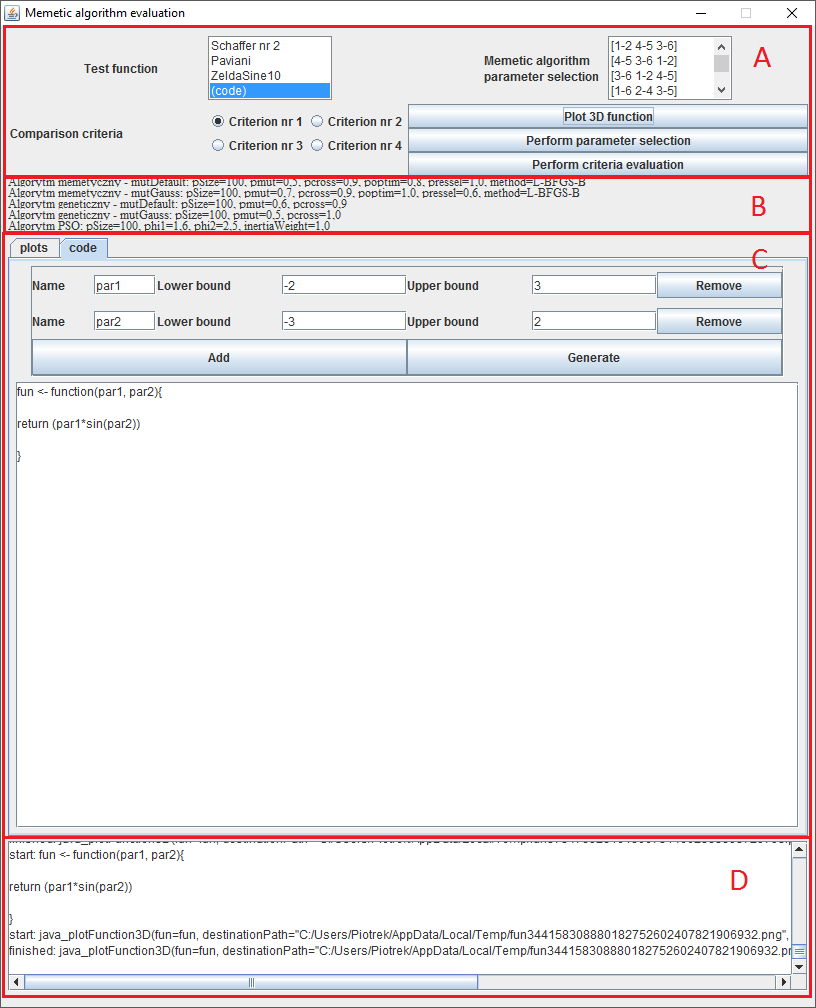
\includegraphics[width=\linewidth]{{img//app01//mockup-with-parts.png}}
\caption{Pełny widok aplikacji}	
\label{fig:app01-fullScreen}
\end{figure}

\par
Na rysunku \ref{fig:app01-plotTab} przedstawiono panel prezentujący wykresy generowane przez aplikację. Przyciskami \emph{Previous} i \emph{Next} możliwe jest przeglądanie pełnej historii wykresów od uruchomienia aplikacji. Jest to ważne z uwagi na fakt, że w wynikiem części operacji może być więcej niż jeden wykres jednocześnie. 

\begin{figure}[hbt]
\centering
  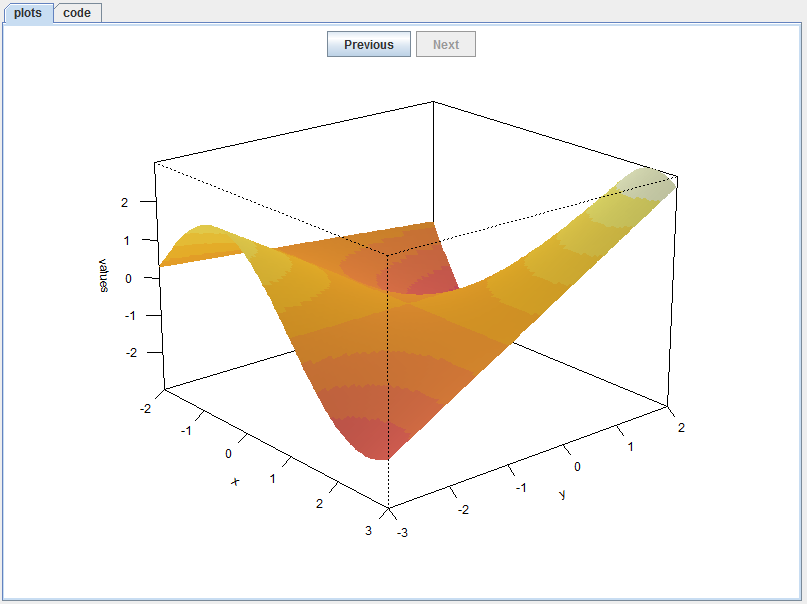
\includegraphics[width=\linewidth]{{img//app01//mockup-plot-tab.png}}
\caption{Zakładka wykresów}	
\label{fig:app01-plotTab}
\end{figure}


